% vim: spell spelllang=en:
%! TEX root = **/00-main.tex

\newcommand{\sssfig}[1]{
    \pagebreak
    \subsubsection{#1}%
    \label{ssub:#1}
}

\newcommand{\hibp}[2]{
    \begin{figure}[H]
        \centering
        \includegraphics[width=0.8\linewidth]{desc-#1-hi_bp}
        \caption{Histogram \& Boxplot of #2}%
        \label{fig:#1}
    \end{figure}
}

\newcommand{\tabn}[2]{
    \begin{table}[H]
        \centering
        \caption{Extended summary statistics of #2}%
        \label{tab:#1}
        \input{../../analysis/tables/desc-#1-ext_sum}
    \end{table}
}

\newcommand{\fign}[2]{
    \sssfig{#2}
    \hibp{#1}{#2}
    \tabn{#1}{#2}
}

\newcommand{\figf}[2]{
\sssfig{#2}
\begin{figure}[H]
    \begin{minipage}{0.49\linewidth}
            \centering
            \includegraphics[width=\linewidth]{desc-#1-bar}
    \end{minipage}
    \begin{minipage}{0.49\linewidth}
            \centering
            \includegraphics[width=\linewidth]{desc-#1-pie}
    \end{minipage}
    \caption{Barplot \& Pie chart of #2}%
    \label{fig:#1}
\end{figure}
\begin{table}[H]
    \centering
    \caption{Table of #2 frequency}%
    \label{tab:#1}
    \input{../../analysis/tables/desc-#1-freq}
\end{table}
}

% Basic statistical descriptive analysis

\section{Basic statistical descriptive analysis}%
\label{sec:basic_statistical_descriptive_analysis}

% Univariate for all the variables included in the study (half a page per variable)
\subsection{Univariate analysis}%
\label{sub:univariate_analysis}

%\begin{comment}

\begin{table}[H]
    \centering
    \caption{Numerical variables summary}%
    \label{tab:num_summary}
    \resizebox{\linewidth}{!}{%
    
\begin{tabular}[t]{llllllll}
\toprule
  & Min & 1st Q. & Median & Mean & 3rd Q. & Max & NA's\\
\midrule
host\_listings\_count & 0.00 & 1.00 & 2.00 & 16.81 & 11.00 & 551.00 & 8\\
accommodates & 1.000 & 2.000 & 2.000 & 3.297 & 4.000 & 16.000 & NA\\
bedrooms & 1.000 & 1.000 & 1.000 & 1.604 & 2.000 & 16.000 & 684\\
beds & 0.000 & 1.000 & 2.000 & 2.233 & 3.000 & 48.000 & 409\\
price & 0.00 & 35.00 & 55.00 & 86.34 & 95.00 & 10000.00 & NA\\
\addlinespace
minimum\_nights\_avg\_ntm & 1.00 & 1.40 & 2.70 & 10.67 & 12.10 & 1123.00 & NA\\
maximum\_nights\_avg\_ntm & 1.000e+00 & 3.300e+02 & 1.125e+03 & 3.118e+05 & 1.125e+03 & 2.147e+09 & NA\\
availability\_30 & 0.00 & 0.00 & 24.00 & 17.55 & 30.00 & 30.00 & NA\\
availability\_60 & 0.00 & 0.00 & 52.00 & 36.43 & 59.00 & 60.00 & NA\\
availability\_90 & 0.00 & 3.00 & 80.00 & 56.01 & 89.00 & 90.00 & NA\\
\addlinespace
availability\_365 & 0.0 & 55.0 & 180.0 & 191.3 & 352.0 & 365.0 & NA\\
number\_of\_reviews & 0.0 & 0.0 & 5.0 & 33.1 & 36.0 & 743.0 & NA\\
number\_of\_reviews\_ltm & 0.000 & 0.000 & 1.000 & 6.401 & 9.000 & 278.000 & NA\\
number\_of\_reviews\_l30d & 0.0000 & 0.0000 & 0.0000 & 0.1621 & 0.0000 & 15.0000 & NA\\
review\_scores\_rating & 20.00 & 88.00 & 93.00 & 91.08 & 98.00 & 100.00 & 5971\\
\addlinespace
review\_scores\_accuracy & 2.000 & 9.000 & 10.000 & 9.379 & 10.000 & 10.000 & 5982\\
review\_scores\_cleanliness & 2.000 & 9.000 & 9.000 & 9.227 & 10.000 & 10.000 & 5980\\
review\_scores\_location & 2.000 & 9.000 & 10.000 & 9.618 & 10.000 & 10.000 & 5985\\
review\_scores\_value & 2.000 & 9.000 & 9.000 & 9.055 & 10.000 & 10.000 & 5985\\
reviews\_per\_month & 0.010 & 0.210 & 0.710 & 1.179 & 1.770 & 21.410 & 5731\\
\bottomrule
\end{tabular}
}
\end{table}

\Cref{tab:num_summary} shows an overview of the numerical variables statistics.


\fign{accommodates}{Accommodates}
% Use this to not pagebreak from subsection

%\subsubsection{Accommodates}%
%\label{ssub:accommodates}
%\hibp{accommodates}{Accommodates}
%\tabn{accommodates}{Accommodates}

In the boxplot we can that there are some outliers. However the distribution of
the variable seems to be in line with socioeconomic distributions. The majority
of listing have low to medium capacities (small-medium houses), while there's
only a fraction of high capacities (big houses).


\fign{bedrooms}{bedrooms}

The majority of listing contains between 1-4 bedrooms, being the mean around
1.6. There are some outliers, but they can somewhat be explained due to the same
reasons mentioned in the accommodates analysis.


\fign{beds}{beds}

The distribution of beds and the outliers seem to follow a similar distribution
as bedrooms.  This is to be expected as those to variables should be correlated.


\fign{availability_30}{availability 30}

If we look at the availability in the next 30 days after the data was taken, we
can clearly see some polarization. There are some rentals with 0 available days
and some close to all days. This polarization explains the high variance of this
variable.


% TODO: ho posem a l apendix?
\fign{availability_60}{availability 60}

For the availability in the coming 2 months the distribution of data
follows an almost identical pattern to the availability in the next
30 days, where many listings don't have any availability and the rest
are hardly occupied. The high proportion of properties with no
availability could be explained by the fact that on \airbnb
you can have a listing up that isn't open for rental and thus isn't
available.

\fign{availability_90}{availability 90}

The availability for the following 90 days again has practically
the same distribution and we believe the same reasons explain it.

\fign{availability_365}{availability 365}

The availability of the year follows a similar distribution to the monthly one.
The only difference are some peaks at 90 days and half a year, which both are
likely numbers for a host to rent its listing.


\figf{host_acceptance_rate_cat}{host acceptance rate cat}

Up to 66\% of the hosts have a very high chance of accepting a customer. There
is a large number of \emph{NA}'s as well.


\figf{host_has_profile_pic}{host has profile pic}

As seen in \cref{fig:host_has_profile_pic}, over 99\% of host with
listings in Barcelona have a profile picture, in fact only 55 out of 20,476
hosts don't have a picture. Therefore, we don't expect this variable to provide
significant insight into answering the question we are posing.

\figf{host_identity_verified}{host identity verified}

\Cref{fig:host_identity_verified} shows that only 74\% of hosts have had
their identity verified by \airbnb, meaning that the other 25\% isn't.  This can
be expected since the verification process can be complicated in some cases,
even requiring the host to provide an official document or additional pictures
of himself.

\figf{host_is_superhost}{host is superhost}

As seen in \cref{fig:host_is_superhost}, only the 19\% of hosts are superhosts.
This may be the case because the conditions to achieve this status are rather hard.

\fign{host_listings_count}{host listings count}


\Cref{fig:host_listings_count} shows that the majority of hosts only have a
small amount of listings, being the median 2. However we can see that there is a
lot of variability with many outliers. These outliers might correspond to
businesses that own lots of listings.

\fig{desc-host_listings_count-hi_bp-tallat100}{host listings count}

In \cref{fig:desc-host_listings_count-hi_bp-tallat100} we can observe, which we couldn't in figure \Cref{fig:host_listings_count}, that
the most common number of listings is one, which is to be expected.

\figf{host_response_rate_cat}{host response rate cat}

This variable conveys how attentive the host is, as it tells us to what degree
the host replies to messages received inquiring about its listings. As seen in
\cref{fig:host_response_rate_cat}, 55\% of hosts have a very high
response rate, that is they reply to more than 80\% of messages they receive.
It should be noted that this variable has a high share of "Unknown" 
data, approximately 34\%.


\figf{host_response_time}{host response time}

\Cref{fig:host_response_time} shows that the quicker the response, the more
number of entries it has. A fact to point out as well is the large number of
\emph{NA}'s.


\figf{host_since_season}{host since season}

To our surprise there number of new hosts listings remain more or less equal over
the four seasons. In \cref{fig:host_since_season} we can see that Spring/Summer
still have a bigger influx but not as much as we had initially hypothesised.


\figf{host_since_year}{host since year}

In \cref{fig:host_since_year} we can see that except for the first years the
among of new hosts has more or less remained constant. However in 2019 there has
been another spike of new hosts.


\figf{instant_bookable}{instant bookable}

As seen in \cref{fig:instant_bookable} there are nearly as many
instant bookable listings as not.

%\end{comment}

\fign{maximum_nights_avg_ntm}{maximum nights avg ntm}

\Cref{tab:maximum_nights_avg_ntm} shows that the median for
the maximum number of nights a listing can be booked is 1,125.
This doesn't come as a surprise as 1,125 nights is the maximum
\airbnb allows the host to set. Understandably, hosts set it to the
maximum as they don't want to limit themselves. Interestingly, 
there seems to be a few hosts that have set the maximum to less
than 50 days, which could make sense in the case they only want to
rent their properties during the holidays for example.



\fign{minimum_nights_avg_ntm}{minimum nights avg ntm}

As expected, most listings have their minimum nights stay set to 1.
Any other distribution of data would have been
unanticipated as it makes sense to have a minimum of 1 so as to avoid
losing any potential tenants. 

\figf{neighbourhood_group_cleansed}{neighbourhood group cleansed}

Looking at \cref{fig:neighbourhood_group_cleansed} we can see that
L'Eixample and Ciutat Vella are the most popular neighborhoods for listing.


\fign{price}{price}
\fig{desc-price-hi_bp-tallat500}{price}

In \cref{fig:desc-price-hi_bp-tallat500} we can see that there are some extreme
outliers. To visualize the distribution better we have cut the histogram at
price 500. Having done that we can see that the price distribution seems to
follow a chi-square. We were surprised to find out that the mean price is around
\$86.34.


\fign{review_scores_rating}{review scores rating}

We can see that the majority of reviews are considered positive. The mean in
fact is a 91.07. That would explain why a common technique among renters is to
consider any review lower than 90 as negative.

We can see as well that there is some polarization, being the most common rating
among negative reviews a 0 and the most common among positive a 10. We suppose
polarization occurs because users are more likely to leave reviews when they had
either really good or really bad experiences.


\fign{review_scores_value}{review scores value}

This variable follows a similar distribution as the other reviews seen so far.
Despite that it has the peculiarity of having less perfect scores.


\fign{review_scores_location}{review scores location}

The location score seems to be the one with most positive reviews. In fact the
mean is 9.61, almost 0.5 higher than the overall rating. We found as well very
few negative reviews, being in fact the median and Q3 both a 10.


\fign{review_scores_accuracy}{review scores accuracy}

The distribution of this variable is really similar to the review score ratings.


\fign{review_scores_cleanliness}{review scores cleanliness}

The distribution of this variable is really similar to the review score ratings.


% TODO

\fign{number_of_reviews}{number of reviews}

Some listings don't have any reviews but most do. The median is 5,
which seems reasonable as not all tenants leave reviews. What is
surprising is that there are some outliers with around 600 review,
and not just one but a few. Possibly these are lsitings that have been
up for a long time and on top of that are very popular and thus
are rented very often.

\fign{number_of_reviews_l30d}{number of reviews l30d}

Most listings don't have any reviews in the 30 days prior to
when the data was collected on the 24th of August 2020. 
That is reasonable given that we are
in a global pandemic and tourism has decreased dramatically, therefore
not many \airbnb listings will have been rented and reviewed.


\fign{number_of_reviews_ltm}{number of reviews ltm}

Similarly to the total number of reviews and the number of reviews
over the last 30 days, most listings didn't receive more than one
review. The maximum, however, is 278, which seems implausible given
Covid but technically possible. Therefore we won't count these 
outliers as errors.

\fign{reviews_per_month}{reviews per month}

When looking at \cref{fig:reviews_per_month} we can clearly see a decreasing
curve with its mean around 1.17. We found some outliers with the max number of
reviews per month being 21. Despite it being quite larger than the mean we think
it is still plausible to have 21 reviews over a 30 day span.

\figf{room_type}{room type}

The vast majority of listings correspond to entire homes/apartments or private
rooms.

\pagebreak
% Bivariate when relevant (half a page per pair of variables)
\subsection{Bivariate analysis}%
\label{sub:bivariate_analysis}

\begin{figure}[H]
    \centering
    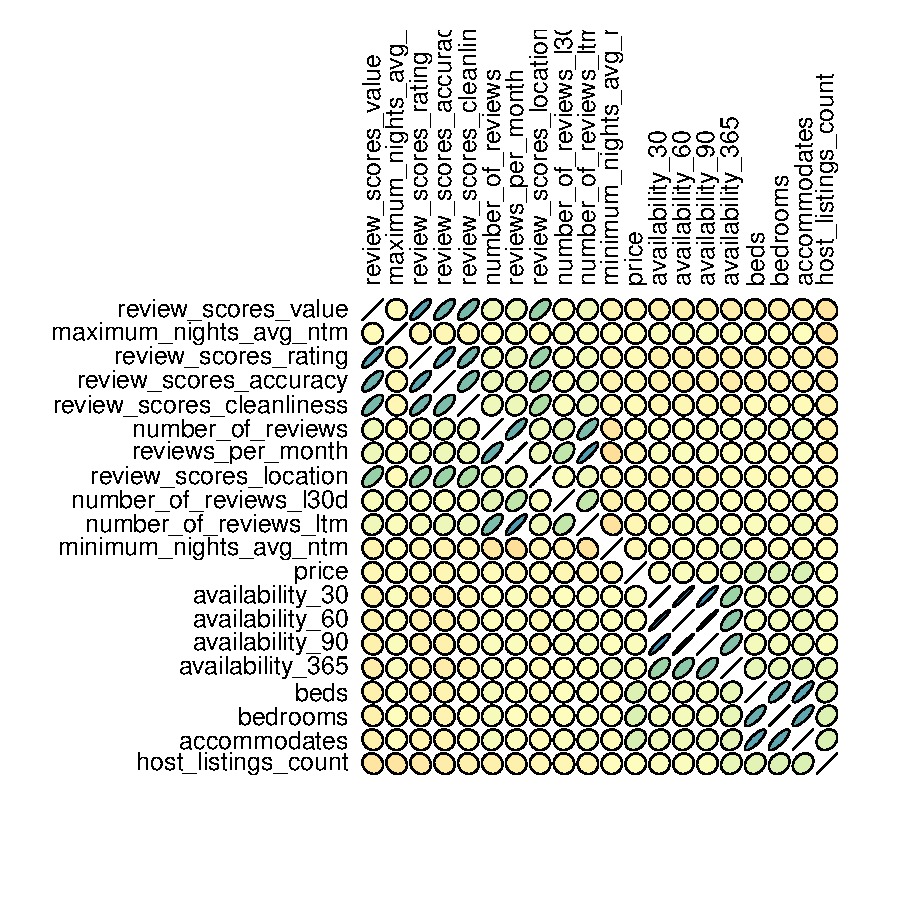
\includegraphics[width=0.7\textwidth]{bivar-ellipse}
    \caption{Ellipses}%
    \label{fig:ellipses}
\end{figure}

We are using \cref{fig:ellipses} to analyse the correlation between variables. The more narrow the ellipsis is the bigger the correlation between variables. Knowing this we can clearly see that there is some correlation between all review scores (review\_scores\_rating,
review\_scores\_cleanliness, review\_scores\_accuracy..). There is some correlation as well between accommodates, bed and bedrooms. All availability variables are really correlated as well.
\subsubsection{Host since year vs host listings count}

\fig{bivar-host_since_year-host_listings_count}{Number of listings depending on the year the host joined Airbnb}



Looking at \cref{fig:bivar-host_since_year-host_listings_count} we can see that
there is no clear correlation between the number of listings a host has and the
time they have been in the platform.It seems like most of the users have a small
amount of listings.

However, the small group that joined the platform in the years 2009, 2010 and
2011 seems to include some owners with upwards of 100 and 150 listings. This
seems to confirm that most of the early adopters of the platform were businesses
or big owners that gathered a lot of buildings. We can also see that some of the
hosts with more listings joined in the recent years, probably joining the
platform after seeing great results from others' operations.


\pagebreak
\subsubsection{Host since year vs price per night}

\fig{bivar-host_since_year-price}{Price per night depending on the year the host joined \airbnb}

Looking at \cref{fig:bivar-host_since_year-price} we can see that again, there
is no relation between the price of the listings and the year the host joined,
there are a few differences on price, all in the neighbourhood of 80-125 dollars
a night, but we also see the same tendency we saw in the last graph, the median
price for the listings posted by hosts who joined during years 2009, 2010 and
2011 seems to be a bit higher than the median price for the hosts who joined in
subsequent years.

\pagebreak

\subsubsection{Host since year vs room type}

\fig{bivar-host_since_year-room_type}{Room type depending on the host's joining year}


What we wanted to find out with \cref{fig:bivar-host_since_year-room_type} was
if there was any initial promotion within a certain group of hosts, something
along the lines of contacting different hotel chains to promote the platform,
which at that time was still small, and give them certain advantages to use
\airbnb.
We would have expected, if that was the case, a significantly bigger share of
the early years' hosts to be listing hotel rooms instead of private rooms or
entire apartments.
This obviously was not the case, which is interesting, since it indicates that
\airbnb did not grow through the kind of techniques we had expected.


\pagebreak
\subsubsection{Number of reviews vs review score rating}

\fig{bivar-number_of_reviews-review_scores_rating}{Score rating vs number of reviews}

 In this case, \cref{fig:bivar-number_of_reviews-review_scores_rating} shows how
 the number of reviews affects the total rating. We can see that when there are
 not many reviews those can be anywhere within range, but once the listings get
 a significant amount of reviews it is harder and harder to find listings with a
 low rating. This, we believe, is due to people's tendency to give polarized
 scores and avoid booking the listings with really low scores.

\pagebreak
\subsubsection{Reviews per month vs review score rating vs price}

\fig{bivar-reviews_per_month-review_scores_rating}{Score rating vs reviews per month}

 To see if there is a difference, we have created
 \cref{fig:bivar-reviews_per_month-review_scores_rating}, which shows how the
 number of reviews per month correlates to the score of the reviews a listing
 has, but also integrating the price of such listing. It is interesting to see
 that some of the most reviewed listings are not very expensive and that the
 tendency that we saw in \cref{fig:bivar-host_since_year-room_type} is still
 there, proving that the listings that get reviewed the most tend to have pretty
 good ratings.

\pagebreak

\subsubsection{Price vs neighbourhood}

\fig{bivar-price-neighbourhood_group_cleansed}{Price of listings depending on the neighbourhood \airbnb}

% TODO: Nose si a la figure "we can see" els mean prices XD
As Barcelona dwellers we know that there are some neighborhoods more expensive
to others. We want to find out if this still holds when talking about \airbnb
rents.  We can see in figure \cref{fig:bivar-price-neighbourhood_group_cleansed}
that for example L'Eixample has a mean price of 96.20, %TODO dollars / euros?
while Nou Barris has a mean price of 41.10.  %TODO dollars / euros?
We can see as well that the high price outliers seem to vary between
neighborhoods. This leads us to believe that although not much there is some
correlation between price and neighborhood.

\pagebreak

\subsubsection{Minimum number of nights vs room type}

\fig{bivar-room_type-minimum_nights_avg_ntm}{Minimum number of nights depending on room type}

From figure \cref{fig:bivar-room_type-minimum_nights_avg_ntm} we can clearly see
that hotel rooms and shared rooms have a minimum average of nights much lower
than the entire homes or private rooms.  We can see that entire homes/apartments
have less variance, being the majority of values concentrated near the mean,
while in the private rooms we can see a much larger interquartile range.

% When required, please include descriptives before and after preprocessing
%\subsection{Conclusion}%
%\label{sub:data-conclusion} % TODO


% Conclude the section with one paragraph describing how is your data
